\documentclass[../all.tex]{subfiles}
\begin{document}
%%%%%%%%%%%%%%%%%%%%%%%%%
\section{Experimentación} % Evaluación
%%%%%%%%%%%%%%%%%%%%%%%%%

\subsection{Problemática lenguaje natural}
El procesamiento del lenguaje natural (PLN o NLP en sus siglas anglosajonas) es una rama de la Inteligencia Artificial encargada de estudiar métodos de comunicación entre máquina y hombre a través del lenguaje natural, es decir, el lenguaje empleado de forma habitual en una conversación escrita u oral entre personas\\ 
El lenguaje natural presenta muchas características que lo hacen un verdadero reto para las ciencias de la computación. Como suele pasar en el mundo de la Inteligencia Artificial, una tarea que puede parecer para una máquina. Aspectos como la ambigüedad, la espontaneidad, la falta de fluidez, las referencias y las abreviaturas son difíciles de procesar.

\subsubsection{Homonimia}
{\color{red} 
    TODO: DEFINICIÓN EJ: BONITO PUEDE SER PEZ O ADJETIVO
}
\subsubsection{Polisemia}
{\color{red} 
    TODO: DEFINICIÓN
}
\subsubsection{Anáfora y elipses}
{\color{red} 
    TODO: DEFINICIÓN
}
\subsubsection{Sintaxis no normalizada}
{\color{red} 
    TODO: DEFINICIÓN
}
\subsubsection{Contexto}
{\color{red} 
    TODO: DEFINICIÓN
}

\subsection{Fase 0 - Extracción de la información}



\subsection{Fase 1 - Clasificación de texto según temática}


\begin{figure}[H]
    \centering
    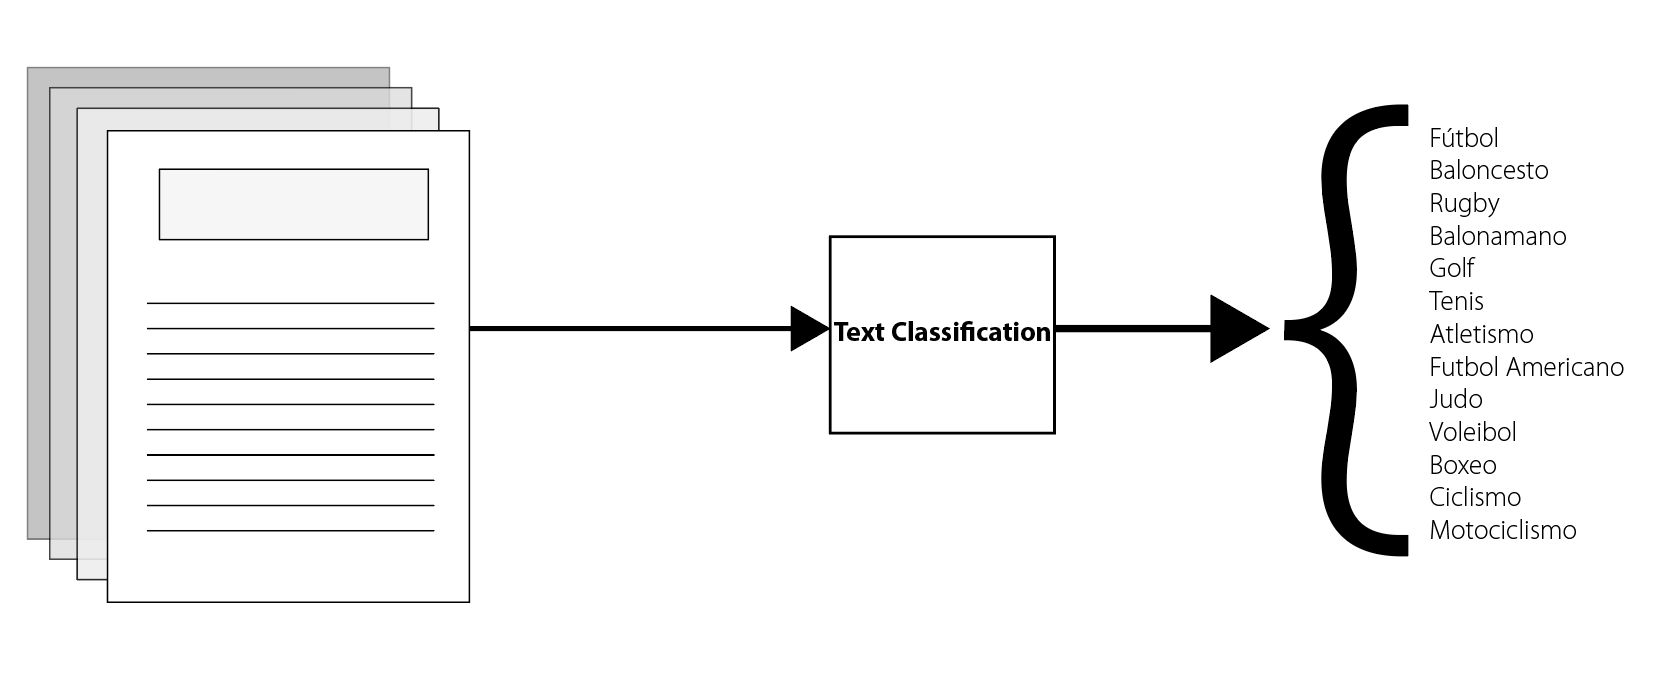
\includegraphics[height=13cm, width=15cm]{imgs/textClassification.png}
    \caption{Idea principal del clasificador de texto}
\end{figure}


Para está primera fase primero se quiso evaluar según el contenido de Wikipedia. Se extrajeron las palabras más repetidas del contenido de cada deporte en Wikipedia. Para ello se quitaron los signos de puntuación y palabras vacías, entendiendo como palabras vacías todos los artículos, preposiciones y números. {\color{red} TODO: adjuntar foto resultado}\\
Con esta técnica se pudo ver que funcionaba bien para clasificar textos grandes como artículos o noticias pero en frases cortas como son los \textit{tweets} no se conseguía una \textit{accuracy} que se pudiera considerar aceptable. Para mejorarlo se decidió hacer una ontología de cada uno de los deportes. En concreto se decidió clasificar las palabras que envolvían un deporte según tres criterios; \textit{key words} que son las palabras que solo se utilizan en un deporte, sus jugadores más destacados y los nombres de sus campeonatos (ej: fútbol; Lionel Messi, bota de oro, etc), \textit{secondary words} que son palabras que se pueden usar en ese deporte pero que pueden referir a algún otro deporte (ej: fútbol; balón, pelota, botas, etc) y por último \textit{excluding words} que son todas las \textit{key words} de los otros deportes y \textit{secondary words} de otros deportes que excluyen (ej: fútbol; manillar, palo de hierro, etc).

Se intento hacer stemmer pero empeorava los resultados, lo probaremos otra vez en analisis del sentimiento
se hizo con wiki, por  diccionario propio y para mejorar los tiempos con diccionario propio y arbol

\begin{figure}[H]
    \centering
    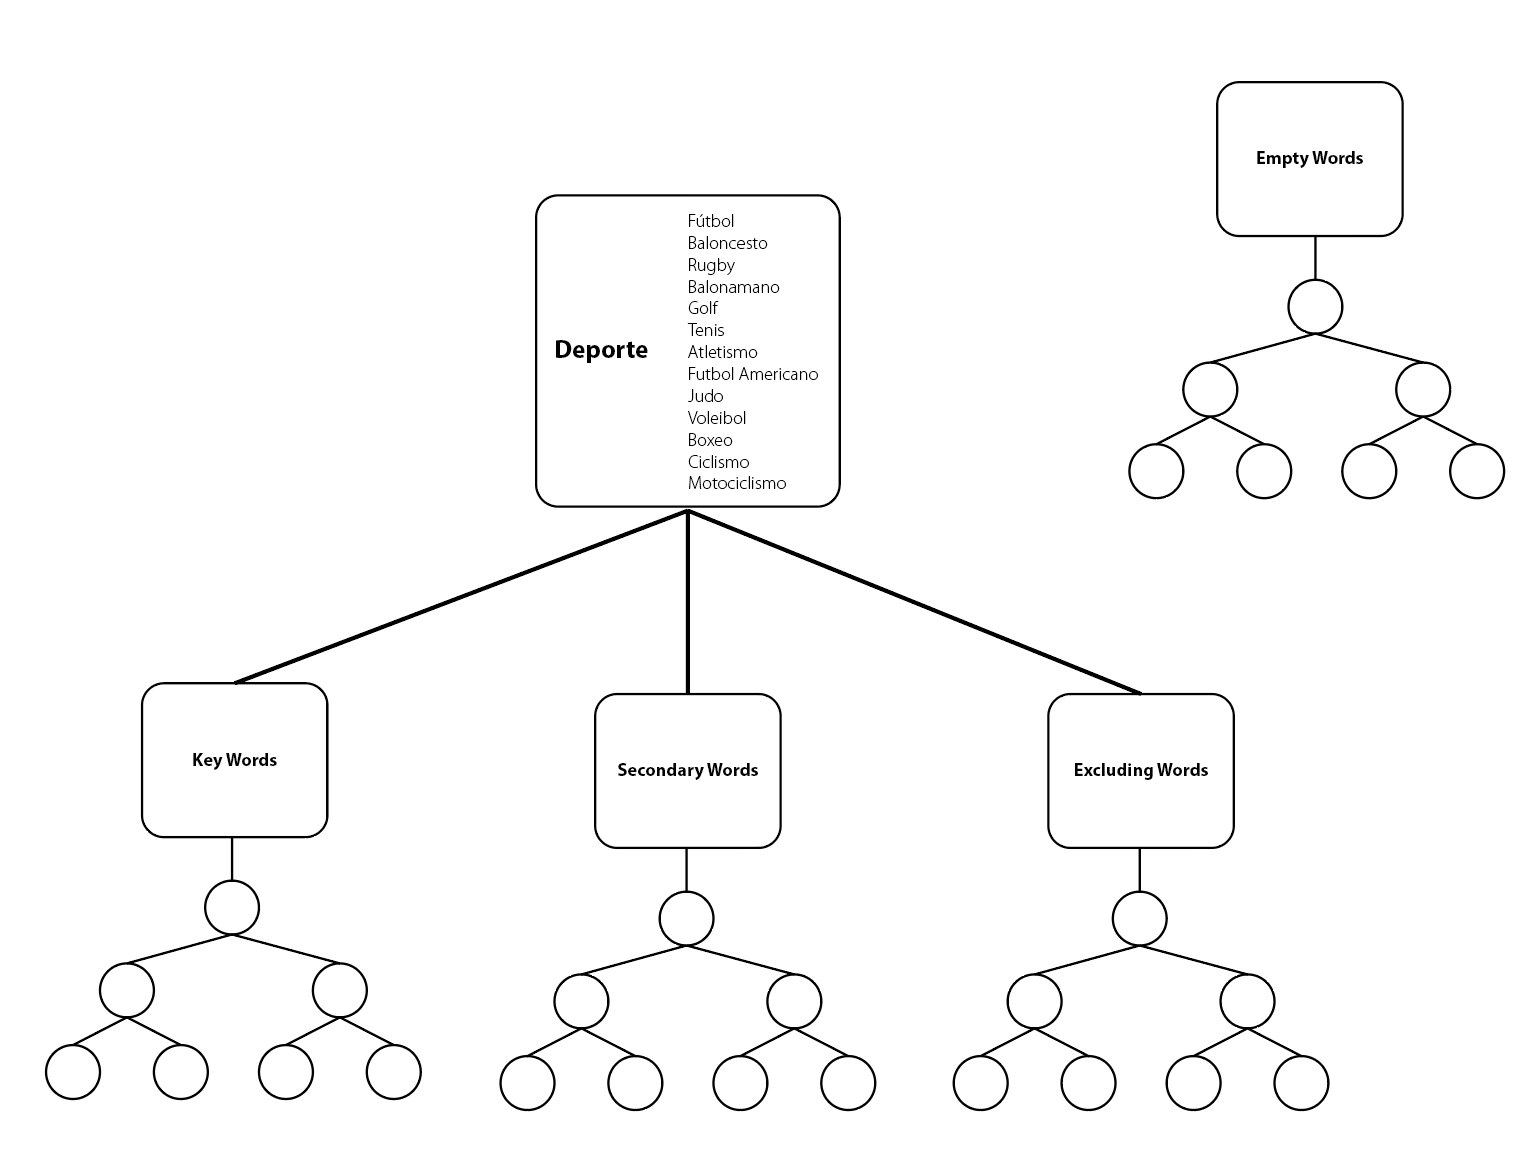
\includegraphics[height=13cm, width=15cm]{imgs/treeScheme.png}
    \caption{Esquema estructuración de los datos}
\end{figure}

{\color{red} 
    TODO: TABLA COMPARATIVA DE LOS METODOS
}
\newpage
\subsection{Fase 2 - Análisis del sentimiento}
    El análisis de sentimiento de textos en las redes sociales (que adopta diferentes nombres en inglés como sentiment analysis, opinion mining, brand monitoring, buzz monitoring, online anthropology, market influence analytics, conversation mining, online consumer intelligence, user generated content) es el proceso que determina el tono emocional que hay detrás de una palabras determinadas, si una frase contiene una opinión positiva o negativa sobre un producto, marca, institución, organización, empresa, evento o persona.\\
    Palabras difíciles
    Los sentimientos se clasifican en positivos, negativos o neutros. Sin embargo, el lenguaje natural es complejo y ambiguo por lo que enseñar a una máquina a que analice los diferentes matices gramaticales, variaciones culturales, jergas, expresiones coloquiales o a distinguir faltas de ortografía, la sinonimia o la polisemia dentro de un contexto que determina el tono de la conversación es francamente difícil. Así, por ejemplo, ante un comentario sarcástico, la máquina tomaría la frase como algo positivo en vez de algo negativo o expresiones como “LOL, OMG, estuvo geeeeeeeniaaaaaaaal” son dificilísimas de procesar.

\newpage
\subsection{Fase 3 -}

\url{http://www.outono.net/elentir/2013/02/02/twitter-5-formas-de-identificar-a-un-troll-y-5-consejos-para-librarte-de-el/}
\url{https://www.fucsia.co/opinion/blogs/entrada-blog/como-detectar-mentiras-internet/35060}
\url{https://www.biobiochile.cl/noticias/2013/09/16/3-senales-para-detectar-cuando-te-mienten-en-facebook-o-whatsapp.shtml}
\url{https://www.elconfidencial.com/tecnologia/2014-02-27/pheme-un-detector-de-mentiras-para-las-redes-sociales_94300/}

\end{document}
